\documentclass[11pt]{article}
\usepackage[utf8]{inputenc}
\usepackage[francais]{babel}
\usepackage[T1]{fontenc}
\usepackage{graphicx}
\usepackage{lmodern}
\usepackage{url}
\usepackage{underscore}
\usepackage{array}
\usepackage{float}
\usepackage{listings}
\usepackage{regexpatch}
\usepackage[scale=0.75]{geometry}
\usepackage{color}
\usepackage{bigcenter}

\graphicspath{{../images/}}

\title{\textbf{Business Plan}\\{ {\small {\bsc {- Res Publica -}}}}}
\author{Fabien \bsc{Buisson} - Ravi \bsc{Pachy}}
\date{Février 2014}

\begin{document}

\renewcommand{\contentsname}{Sommaire}
\maketitle
\thispagestyle{empty}

\newpage

\tableofcontents

\newpage
\pagestyle{headings}

\section{Présentation}
\label{sec:presentation}
En dernier

% subsection section name (end)

% section Contexte, historique (end)

\section{Équipe \& fonctions}
\label{sec:equipe_fonctions}

\subsection{Introduction}
\label{sub:equipe_intro}
Pour le bon fonctionnement de l'entreprise nous n'aurons pas besoin d'une quantité importantes d'employés. Cependant certaines fonctions sont indispensables, une base salariale en découle donc.
% subsection Introduction (end)

\subsection{Webmaster}
\label{sec:webmaster}
Sera en charge de la réalisation et de la maintenance du site web et permettra le développement d'applications servant à l'entreprise.

% subsection Webmaster (end)

\subsection{Chargé de communication}
\label{sec:communication}
Sa mission sera d'obtenir des contrats directement avec l'habitant ou l'organisme. Il devra avoir préalablement étudier la région afin de proposer et répondre au mieux aux attentes de la clientèle, ainsi qu'être au courant des dernières méthodes et materiaux utilisés.

% subsection Chargé de communication (end)

\subsection{Veille}
\label{sec:}
\subsubsection{Technologique}
\label{ssub:}
L'objet d'une veille technologique sera primordia afin de pouvoir entrer en contact avec les meilleurs fournisseurs dans les différentes région d'action. Une étude régulière dans les différents secteurs (panneaux solaire, eoliennes...) devra être rigoureuse, le but étant de proposer le meilleur du marché, connaitre les avantages et inconvenients de chaque ressource est indispensable.

% subsubsection  (end)

\subsubsection{Fournisseurs}
\label{ssub:}
La recherche de fournisseurs en ressource se réalisera toujours en fonction de la région ciblée. Une étude sur les fournisseurs locaux, ou dans les régions alentours, se réalisera après avoir pris connaissance des meilleurs produits sur le marché actuel. Suite à un trés bon rapport qualité/prix, nous serons en mesure de proposer le meilleur du marché à des prix trés abordable.

% subsubsection  (end)
% subsection Veille (end)

\subsection{Resources humaines}
\label{sec:rh}
Le responsable des ressources humaines aura pour mission de recruter de la main d'oeuvre locale. Un contrat dans une région permet d'employer élécritien(s), plombier(s), maçon(s), agriculteur(s).., parmis les intérimaires locaux.
% subsection Resources humaines (end)

\subsection{Comptable}
\label{sec:}
Gestionnaire de toutes les dépenses et les recettes. Achat de fournitures de bureau, paiement des salaires, vente/achats de produits…, il contrôle tous les mouvements d’argent. En fin d’année, il élabore le bilan comptable de l’entreprise. 
% subsection Comptabilité (end)

\subsection{Demos politis}
\label{sec:}
Aide à la création des assos (statuts figés, supports, contacts, documents type)
Dialogue avec elles (gestion des sous communs)
Aide à la réalisation de projets pour tout le monde
% subsection Demos politis (end)

\subsection{Dirigeant}
\label{sec:dirigeant}
Ce rôle est strictement encadré par les limites et compétences qui lui sont attribuées par les instances décisionnaires de l'entreprise. À l'intérieur de ce cadre, le chef d'entreprise dispose d'une marge d'initiative pour diriger et conduire l'entreprise.
Il défend les intérêts des propriétaires de l'entreprise, mais aussi ceux des parties prenantes à l'entreprise (notamment les salariés et les prestataires de service oeuvrant pour elle)
Il défend aussi un collectif plus élargi pouvant comprendre les parties prenantes externes comme les fournisseurs et  les clients de l'entreprise.
% subsection Dirigeant (end)

% section Équipe & fonctions (end)

\section{Ressources matérielles}
\label{sec:ressources}
L'entreprise aura besoin de diverses ressources matérielles, que ce soit pour la communication dans un premier temps, mais aussi au niveau des locaux et de leurs amménagements. 
Au niveau informatique, Res-Publica travail avec des logiciels libre, (LibreOffice, Latex, Gimp..)
L'amménagement des locaux comptera des bureaux, chaises, ordinateurs et toutes les fournitures de bases qui permettront le bon déroulement du lancement de la société (papier, classeurs, stylos, surligneur, enveloppe...).

Au niveau du site web et du ou des serveur applicatifs qu'aura besoin l'entreprise nous passerons par OVH, qui nous permet de régler pas mois la location des serveurs, et le nom de domaine.
Voici une liste exhaustive des dépenses à fournir : \\
\begin{figure}[h]
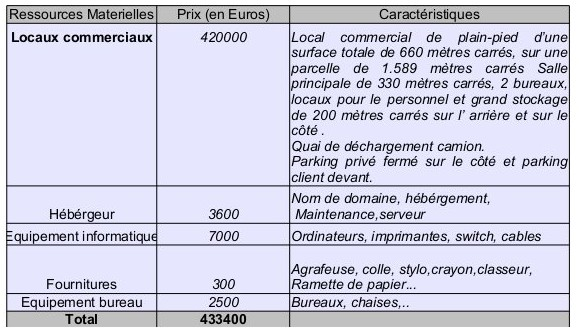
\includegraphics[scale=0.50]{BP.jpg}
\end{figure}


% section Ressources (end)

\section{Étude du marché}
\label{sec:marche}

\subsection{Objectif de l'entreprise}
\label{sec:objectifs}

L'entreprise se propose de jouer le rôle d'une structure coordinatrice pour :
\begin{itemize}
	\item la livraison \og{}clé en main\fg{~}de solutions autonomisantes d'un point de vue alimentaire et énergétique
	\item l'initiation et le financement de projets sociaux et culturels publics
	\item le développement de l'économie locale et de la vie citoyenne
\end{itemize}


% subsection Objectif de l'entreprise (end)

\subsection{Clients}
\label{sub:client}
Les clients visés sont des habitants de villages avec de préférence une petite parcelle de terrain cultivable (potager).
Le terrain étant nécessaire pour l'installation des solutions de chauffage, et de culture notamment.
Puis, compte tenu de la situation géographique, l'entreprise étudiera et proposera diverses solutions. Panneaux solaires pour les régions ensoleillée (Sud) et système de récupération des eaux de pluie pour les plantations dans les régions pluivieuses.
% subsection Clients (end)

\subsection{Stratégie}
\label{sub:strategie}
on prospecte\\
La communication sera un point essentiel. Le lancement repose sur les chargés de communication qui devront présenter le projet en local. Il sera appuyé par de la documentation concrète \\
on installe\\
L'embauche de la main d'oeuvre se fera principalement des les boites d'interim locales en premier lieu puis, suivant les besoins, moins localement. \\
on redistribue\\
Les bénéfices récoltés suites à une ou plusieurs installations seront redistribuées aux différents pôles sociaux culturels créés par la suite ou alors directement à la mairie des communes ayant recourus à nos services. Cette répartition se calculera en fonction du nombre de personnes ayant fait appel à l'entreprise. Plus une commune à eu besoin de nos service, plus nous lui fourniront des aides pour divers projets sociaux culturels.
% subsection Stratégie (end)

% section Marché (potentiel, stratégie, …) (end)

\section{Financier (futur et éventuellement passé)}
\label{sec:financier}
Compte tenu du fait que le smic en 2014 est de: 1 445,38/mois soit 9,53/h, il nous faut calculer la somme salariale des employés de l'entreprise à temps plein
% section Financier (futur et éventuellement passé) (end)

\section{Juridique}
\label{sec:juridique}
\subsection{Forme juridique et capital}
\label{sub:juridique_capital}

La société « Res-Publica » est soumis à un aspect juridique qui est celui d'une SARL (Société à responsabilité limité). Cette SARL comptera trois associés et sera ouvert à plusieurs autres associés. Le capital sera librement déterminé dans les statuts. Il y aura une possibilité de libération de 20 \% lors de la souscription, le solde dans les cinq ans (loi du 15 mai 2001).

La responsabilité de chacun des associés sera limitée au montant de leurs apports respectifs, sauf exception pour les dirigeants de droit ou de fait (violation des statuts, fautes de gestion etc..) et si des garanties personnelles ont été données.
Les associés n'ont pas la qualité de commerçant.
La cession de parts est libre entre associés, réglementée vis à vis des tiers.
Le commissaire aux comptes est non obligatoire (sauf dépassement de certaines limites). Le dépassement des limites à la clôture d'un exercice pour deux des trois critères suivants :
\begin{itemize}
	\item Total du bilan (1 550 000 euros) 
	\item Montant HT du chiffre d'affaires (3 100 000 euros)
	\item Nombre moyen de salarié (100)
\end{itemize}

Les décisions seront prises à la majorité en Assemblée générale. (51\% du capital pour décisions ordinaires, 2/3 du capital pour décisions extraordinaires). (Sauf dérogations contraires prévues par les statuts). En contre partie, les frais de constitution (rédaction des statuts et formalités) seront à la charge de l'entreprise ainsi que les procédure « lourde » de fonctionnement (tenue obligatoire des assemblées, modifications statutaires soumises aux formalités de publicité légale).

Le montant estimé de la société s'élève à environ ????%TODO%???? euros.
% subsection juridique_capital (end)
\subsection{Représentants légaux}
\label{sub:representants}

Les représentants légaux de cette compagnie étant :
\begin{itemize}
	\item Fabien BUISSON domicilié à Marseille (France)
	\item Ravi PACHY domicilié à Marseille (France)
\end{itemize}

% subsection representants (end)

\subsection{Date de création}
\label{sub:date_creation}
La société a été constitué en 2014.
% subsection date_creation (end)



% section Juridique (end)

\section{Création de l'entreprise}
\label{sec:creation_entreprise}

\subsection{Locaux}
\label{sub:locaux}

La domiciliation de l'entreprise correspond à l'adresse administrative de l'entreprise, qui doit être déclarée au CFE et qui figure sur les documents commerciaux de l'entreprise. La domiciliation ne modifie pas la destination du local, qui demeure un local affecté à l'habitation.

Dans une ville de moins de 200 000 habitants l'entreprise pourra être domiciliée chez un des fondateurs si aucune disposition contractuelle ou législative ne s'y oppose (clause du bail excluant expressément la possibilité de domiciliation). Les fondateurs peuvent exercer leur activité chez eux, si aucune disposition contractuelle ou législative ne s'y oppose (clause du bail ou du règlement de copropriété interdisant l'exercice d'une activité professionnelle dans le local).

Si le logement n'est pas situé au rez-de-chaussée, l'exercice d'une activité est possible si :
\begin{itemize}
	\item aucune disposition du bail ou du règlement de copropriété ne s'y oppose
	\item il s'agit de la résidence principale du créateur,
	\item l'activité est exercée exclusivement par les occupants du logement,
	\item l'exercice de l'activité ne conduit pas à recevoir une clientèle ou des marchandises.
\end{itemize}

Si le logement est situé au rez-de-chaussée, l'exercice d'une activité est possible  si :
\begin{itemize}
	\item aucune disposition du bail ou du règlement de copropriété ne s'y oppose
	\item il s'agit de la résidence principale du créateur
	\item l'activité est exercée exclusivement par les occupants du logement
	\item l'exercice de l'activité n'occasionne pas de nuisances ou de danger pour le voisinage, et ne conduit pas à un désordre pour l'immeuble \\
\end{itemize}

Cas particulier du dirigeant demeurant au rez-de-chaussée d'une HLM : l'exercice d'une activité professionnelle peut être autorisée par le Maire de la commune concernée, après avis de l'organisme gestionnaire du HLM.
Le siège de l'entreprise doit se trouver en dehors des grandes villes afin de toucher le plus grand nombre de population rurale possible.\\
Nous optons pour un lieu dans la région de l'Ardèche dans la commune d'Aubenas, endroit propice à la prospection car proche des campagnes, mais aussi stratégique car il est proche des grands axes permettant le transport de marchandises, mais à l'exterieure aux grande villes. Aubenas est donc le lieu adéquat avec l'autoroute A7 qui rend facile l'accès aux grandes métroples comme Lyon, Marseille, Montpellier... .\\
% subsection Locaux (end)

\subsection{Assurance}
\label{sub:assurance}
Afin de protéger l'entreprise, le chef d'entreprise et ses collaborateurs, les biens de l'entreprise, mais aussi les tiers, il est primordial de souscrire une assurance entreprise, que celle-ci soit obligatoire ou non. Cette assurance permet de couvrir les risques qui ne peuvent pas être supportés par la trésorerie et qui pourraient entrainer la faillite.

En souscrivant une assurance, l'entreprise sera protéger des :
\begin{itemize}
	\item dommages qu'elle peut subir
	\item dommages qu'elle peut causer aux tiers
\end{itemize} 

Afin de choisir une assurance, une évaluation des risques encourus et leurs conséquences financières sera réalisée dès sa création. L'assurance peut être souscrite pour l'entreprise et son activité, les personnes de l'entreprise que ce soit le chef d'entreprise ou ses collaborateurs et salariés, ou encore ses biens tels que les locaux ou véhicules.\\

\subsubsection{Inventaire des risques}
\label{ssub:inventaire_risques}
\begin{itemize}
	\item Endettement (aucune poursuite sur patrimoine personnel possible pour des dettes contractées par l'entreprise. Le seul risque est la perte des sommes apportées lors de la création de la société).
	\item Retards accidentels dans une prestation
	\item Défaut de performance
	\item Violation de droits de propriété intellectuelle
	\item Incendie
	\item Perte ou vol de matériels
	\item La retraite
	\item La prévoyance
	\item Plan de licenciement\\
\end{itemize}
% subsubsection inventaire_risques (end)

Voici à titre indicatif quelques exemples de tarifs d'assurance :
\begin{itemize}
	\item Complémentaire santé à partir de 200 euros l'année
	\item Protection juridique	à partir de 100 euros l'année
	\item Assurance perte d'exploitation à partir de 300 euros l'année
	\item Mutlirisques professionels à partir de 400 euros l'année
	\item Garantie décénnale bâtiment à partir de 600 euros l'année
	\item Responsabilité civile à partir de 100 euros l'année
\end{itemize} 


% subsection assurance (end)

\subsection{Communication}
\label{sub:communication}
La campagne de communication nécessite au préalable une élaboration de divers documents officiels. Carte de visite et brochure de présentation sont indispensable lors de la phase de prospection. Le site web permettra aux clients d'avoir accès à tout les renseignements nécessaire et de prendre facilement et rapidement contact avec l'entreprise.
% subsection communication (end)

\subsection{Recrutement}
\label{sub:recrutement}
\subsubsection{Recrutement durable}
label{sub:recrutement_durable}
Le recrutement des employés à long terme qui se verront attribués les diverses fonction cités dans le point \emph{"Équipe \& fonctions"} s'effectuera via divers cabinet de recrutement, appel d'offre, recherche de candidats, afin de permettre l'ajout d'éléments compétents et motivés au sein de l'entreprise.
% subsection recrutement_durable (end)

\subsubsection{Recrutement à court ou moyen terme}
\label{sub:recrutement_court_moyen_terme}
Le recrutement à court ou moyen terme correspond à la main d'oeuvre. Suivant le contrat, la quantité d'installation demandée par les différents clients variera, la main d'oeuvre sera donc variable autant en nombre qu'en temps de travail.
L'entreprise passera par les boites d'intérim locales,pour trouver les plombiers, éléctriciens, maçons,..., dans un premier temps. Puis, selon les contrats et la main d'oeurve à embaucher et qu'au niveau local la main d'oeuvre n'est pas suffisante, l'entreprise se chargera d'entrer en contact avec les boites d'intérim des régions alentours à celle ciblée pour les diverses installations.
% subsection recrutement_court_moyen_terme (end)

% subsection recrutement (end)

\subsection{Comptabilité \& Gestion}
\label{sub:comptabilité_gestion}
La mise en place de journaux officiels est prévu, tels qu'un journal des recettes afin de gérer au mieux la comptabilité, un livre d'inventaire pour gérer les stocks de marchandises et des registres d'immobilisations et amortissements
% subsection  comptabilité_gestion (end)

\subsection{Actions commerciales}
\label{sub:actions_commerciales}

% subsection actions_commerciales (end)

\subsubsection{Echéances fiscales}
\label{ssub:echéance_fiscales}

Impôt sur les bénéfices dépend de la structure juridique choisie 
\begin{itemize}
	\item Impôt sur les sociétés (IS)
	\item Impôt sur le revenu (IR) \\
\end{itemize}

%////////////////////////////////////////%
%////////////////////////////////////////%
%| Mode de détermination  du bénéfice   |%
%////////////////// TODO ////////////////%
%////////////////////////////////////////%

La TVA qui s'élève à 20\% sera facturée au client puis reversée au Trésor Public.
% subsubsection echéance_fiscales (end)

\subsubsection{Croissance}
\label{ssub:croissance}
Pour le bon fonctionnement de l'entreprise, nous nous verrons dans l'obligation de contrôler la croissance afin d'éviter ainsi un effet tunel, et prévoir tout les cas qui seraient défavorables.
Il faudra donc éviter certaines défaillances :
\begin{itemize}
	\item Insuffisance de capitaux propres : pas de "panneaux solaires" pour imprévus (stocks..)
	\item Charges trop élevées par rapport au CA (salaires, frais généraux,...)
\end{itemize}
En contrepartie l'entreprise devra :
\begin{itemize}
	\item Prendre connaissance des prix de revient
	\item Limiter les frais fixes
	\item Surveiller les postes clients et fournisseurs
	\item Suivre les prévisions
\end{itemize} 
% subsubsection croissance (end)

\subsubsection{Développement}
\label{ssub:developpement}
Gérer = Prévoir
Chef d’entreprise 
prendre du recul sur le quotidien
Faire des choix stratégiques : diversification, spécialisation
Changer de structure juridique
S’associer
% subsubsection developpement (end)

% section  Création de l'entreprise (end)

























\end{document}